\section{Old men shall dream dreams}

\begin{quotex}
And it will come to pass after these things that I will pour out My spirit upon all flesh; and your sons and your daughters shall prophesy, your old men shall dream dreams and your young men shall see visions. 
\flright{\textsc{Joel 2:28}} 

\end{quotex}
\paragraph{Mundus Imaginalis}

The visionary \textbf{Emmanuel Swedenborg} recognized three modes of being in the world in respect to the ability to recognize spiritual reality. These certainly seem equivalent to the traditional distinction of pneumatic, psychic, and hylic persons.

\begin{itemize}
\item \textbf{Celestial humanity}: sees that everything in the natural world, which is seen by natural sight, corresponds with a higher, celestial reality. 
\item \textbf{Spiritual humanity}: lost that ability, yet retains a vague memory, or perhaps merely a belief, in immaterial reality. 
\item \textbf{Material humanity}: can only see external things in the world. 
\end{itemize}
\textbf{Henry Corbin} calls the higher spiritual knowledge of celestial humanity ``Hierognosis". This gnosis is of the Mundus Imaginalis, the ``imaginal world" (NOT ``imaginary"). He explains it ontological position:

\begin{quotex}
The existence of this intermediate world, mundus imaginalis, thus appears metaphysically necessary; the cognitive function of the Imagination is ordered to it; it is a world whose ontological level is above the world of the senses and below the pure intelligible world ; it is more immaterial than the former and less immaterial than the latter. 

\end{quotex}
This mundus imaginalis is the analogical world described by \textbf{Hermes Trismegistus} in the \emph{Emerald Tablet}:

\begin{quotex}
Quod superius est sicut quod inferius et quod inferius est sicut quod est superius, ad perpetranda miracula rei unius. That which is above is like to that which is below, and that which is below is like to that which is above, to accomplish the miracles of the one thing. 

\end{quotex}
Analogy expresses the correspondence between the celestial prototype and its manifestation below. The 8 petalled lotus at the crown is our connection to the spiritual world, whether to other spirits, angels, or even the Holy Spirit. The 10 petalled lotus of the solar plexus area is the seat of imaginative revelation, whether they come as visions, dreams, or direct message. The latter is inspiritive revelation, descending even as far as the womb.

\begin{wrapfigure}{rt}{.3\textwidth}
 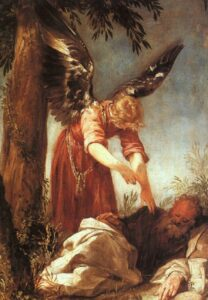
\includegraphics[scale=.5]{a20201025Oldmenshalldreamdreams-img001.jpg} 
 \caption{Elijah's Dream}
 \end{wrapfigure}

\textbf{Mary} had a visit, fully conscious, from the angel Gabriel, and was inspired by the Holy Spirit to sing the Song of Praise.

\textbf{Joseph} was visited by an angel in a dream.

The \textbf{Shepherds} had visions of the shining glory of God and angels.

\paragraph{Dreams}
There are 21 dreams recorded in the Bible, so they are not easily dismissed as sources of insight or revelation.  The writings of the Fathers in the Philokalia offer some comments about dreams.

For example, \textbf{St Diadochos of Photiki} has this advice:

\begin{quotex}
The dreams which appear to the soul through God's love are unerring criteria of its health. Such dreams do not change from one shape to another; they do not shock our inward sense, resound with laughter or suddenly become threatening. But with great gentleness they approach the soul and fill it with spiritual gladness. As a result, even after the body has woken up, the soul longs to recapture the joy given to it by the dream.

There are, however, times when even good dreams do not bring joy to the soul, but produce in it a sweet sadness and tears unaccompanied by grief. But this happens only to those who are far advanced in humility. 

\end{quotex}
Demonic dreams have a different feel:

\begin{quotex}
Demonic fantasies, however, are just the opposite: they do not keep the same shape or maintain a constant form for long. For what the demons do not possess as their chosen mode of life, but merely assume because of their inherent deceitfulness, is not able to satisfy them for very long. 

\end{quotex}
Diadochos recommends that beginners not pay much attention to dreams:

\begin{quotex}
In our quest for purity the safest rule is never to trust to anything that appears to us in our dreams. For dreams are generally nothing more than images reflecting our wandering thoughts, or else they are the mockery of demons. 

\end{quotex}
While that is true of most dreams which are forgettable, it seems extreme to ignore true revelations. Those are gifts. And one should be particularly attentive to recurring themes in dreams. Even if they don't reveal anything supernatural, they provide insights into our own psyche. Moreover, even the mockery of demons can help us to recognize our impurities and vulnerabilities. Diadochos admits as much:

\begin{quotex}
the intellect, when pure, sometimes even feels joy at having been able to see through their tricks [of demons]; indeed it often challenges them during the dream itself and thus provokes them to great anger. 

\end{quotex}
\textbf{Nikitas Stithatos} also has a warning:

\begin{quotex}
Those who have attained spiritual maturity can also analyze the impulsions and proclivities of the soul, and can guide and guard their inner state, on the basis of dreams. For bodily impulsions and the images in our intellect depend upon our inner disposition and preoccupations. If your soul hankers after pleasure and material things, you will dream about acquiring possessions and having money, about the female figure and sexual intercourse – all of which leads to the soiling and defilement of soul and body. 

\end{quotex}
Therefore, if you have such soul defiling dreams, they are not necessarily demonic. Rather Holy Spirit convicts the believer of sin through such dreams. Therefore, they are gifts that remind us of our shortcomings and where we need improvement. They we may reach the next stage:

\begin{quotex}
Things seen in sleep are true and imprinted on the spiritual intellect in the case, not of everyone, but only of those whose intellect is purified, who have cleansed the soul's organs of perception and who are advancing toward the contemplation of the inner essences of created things. Such people do not worry about day-to-day matters, nor are they troubled about this present life. 

\end{quotex}
\textbf{St Antony the Great} has a deeper understanding of dreams.

\begin{quotex}
Man alone is capable of communion with God. For to man alone among the living creatures does God speak: at night through dreams, by day through the intellect. And He uses every means to foretell and prefigure the future blessings that will be given to those worthy of Him. 

\end{quotex}
The revelation of night is esoteric, revelation by day is exoteric.

\paragraph{Visions}
\begin{quotex}
Where there is no prophetic vision the people cast off restraint \flright{\textsc{Proverbs 29:18}}

I saw in the night visions, and behold, with the clouds of heaven there came one like a son of man, and he came to the Ancient of Days and was presented before him. \flright{\textsc{Daniel 7:13}}

And the Lord said to Paul one night in a vision, Do not be afraid, but go on speaking and do not be silent \flright{\textsc{Acts 18:9}}

\end{quotex}
There are more than 100 references to visions in the Bible, not least of which is Ezekiel's vision and the entirety of Revelation. Nikitas Stithatos offers these comments about visions and the spiritual life:

\begin{quotex}
Visions are constant; the one does not change into another, but they remain imprinted upon the intellect unforgettably for many years. Those that disclose the upshot of things to come, and assist the soul by inspiring it with compunction and the sight of fearful wonders, make the beholder reflective and strike him with awe on account of their constancy and their fearsome nature. Hence they are treated with great seriousness by those skilled in spiritual matters. Revelations occur when the purified and illumined soul is able to contemplate in a way that transcends normal sense-perception. They have the force of things and thoughts miraculous and divine, initiating us into the hidden mysteries of God, showing us the outcome of our most important problems and the universal transformation of things worldly and human. 

\end{quotex}
\textbf{Vladimir Solovyov} documented his three visions of Sophia. He describes them this way:

\begin{quotex}
Visions are involuntary visual images and pictures, received while awake, that produce a more or less complete impression of objective reality, but which do not have any external material substance. Visions arise and are maintained regardless of a subject's own conscious acts, and therefore seem to him like external reality. 

\end{quotex}
Solovyov regarded Jacob Boehme and Swedenborg as the fullest and highest theosophical expression of the old Christianity. However, their world conception was static and ignored the world process. Solovyov's vision led to an understanding of the world process, although he regarded Friedrich Schelling as his predecessor. Schelling himself was influenced by Boehme and Swedenborg.

E F Schumacher in \emph{A Guide to the Perplexed} uses the visionaries \textbf{Jakob Lorber} and \textbf{Edgar Cayce} as examples of the second field of knowledge: the Inner Life.

\paragraph{Sources}

\textbf{Henry Corbin}, \emph{Swedenborg and Esoteric Islam}

\textbf{Judith Kornblatt} and \textbf{Vladimir Solovyov}, \emph{Divine Sophia}

Swedenborg by Vladimir Solovyov: \url{https://www.gornahoor.net/library/SwedenborgByVladimirSolovyov.pdf}

The \emph{Philokalia}

\textbf{E F Schumacher}, \emph{A Guide to the Perplexed}

Every dream in the Bible: \url{https://overviewbible.com/infographic-dreams-bible/}

100 Bible verses about visions: \url{https://www.openbible.info/topics/vision}



\flrightit{Posted on 2020-10-25 by Cologero }
